\documentclass[11pt]{article}
\usepackage[margin=25mm]{geometry}
\usepackage{fontspec}
\usepackage{kotex}
\usepackage{graphicx}
\usepackage{booktabs}
\usepackage{longtable}
\usepackage{hyperref}
\setmainfont{Latin Modern Roman}
\title{RUX 과학 결과 작업 보고서 (초안)}
\author{REI Bianchi 연구 실행 기록}
\date{2026-10-14}
\begin{document}
\maketitle
\noindent\textbf{상태: 작업 보고서 / 과학 admission HOLD.} 권위 계획은 ADOPTED v2 \texttt{REI-ATOMIC-REUSE-RESET-20261012}이며 v2의 17개 의무 및 claim 경계를 보존한다. 이 초안에 포함된 과학 자료는 보존 F08 synthetic/prescribed-discrete paired endpoint 15행의 재표현이다. 새 physical solver 실행은 0회다.
\section{요약}
동일한 $t=10^{13}\,\mathrm{s}$의 저장 F08 BI와 FLRW endpoint를 비교했다. 15행은 7개 resolution별 paired difference를 이룬다. 결과는 합성·처방 이산 모델의 범주형 endpoint 차이다. 중간 시간 history, 물리적 EoR, QV, 하늘 신호 또는 연속체 오차 상계를 주장하지 않는다. 상속된 campaign 상태는 \texttt{PRESCRIBED\_DISCRETE\_PAIRED\_HISTORY\_INDEPENDENT\_PASS}이고 physical/scientific admission은 \texttt{HOLD}다.
\section{방법 및 규약}
저장 CSV의 같은 resolution BI endpoint에서 FLRW endpoint를 뺐다. 과거 계산을 재실행하거나 endpoint 사이의 시간을 보간하지 않았다. 그림의 점은 범주형 비교이고 error bar가 없다. ledger의 기존 \texttt{max\_abs}는 CSV에서 다시 계산한 값이 아니다. 현재 convention contract는 metric $(-,+,+,+)$, $u\cdot u=-1$, proper seconds와 명시된 origin, proper density, $R:\mathrm{m}^{-3}\mathrm{s}^{-1}$, $Q:\mathrm{J}\,\mathrm{m}^{-3}\mathrm{s}^{-1}$ 및 $N=n u\Rightarrow\nabla\cdot N=R/c$, $J=c n u\Rightarrow\nabla\cdot J=R$다. H/He electron census는 선언된 baseline에서 $n_e=n_H[x_{\mathrm{HII}}+f_{\mathrm{He}}(x_{\mathrm{HeII}}+2x_{\mathrm{HeIII}})]$다. Case-A escape에서 emitted recombination photon count는 정의되지 않는다. Unknown remains null; omitted physics is not zero error. 이 conventions 문장은 미결 scenario 입력을 채우지 않는다.
\section{보존된 endpoint 차이}
\begin{center}\small
\begin{tabular}{lrrrr}\toprule
Resolution & $\Delta x_{\rm HII}$ & $\Delta T$ (K) & $\Delta\Gamma_{\rm HI}$ (s$^{-1}$) & $\Delta u_\gamma$ (eV/H)\\\midrule
T0 & $2.852045\,10^{-7}$ & $-0.002130787$ & $8.520161\,10^{-19}$ & $-4.969156\,10^{-6}$\\
T1 & $2.851331\,10^{-7}$ & $-0.002130624$ & $8.520641\,10^{-19}$ & $-4.967761\,10^{-6}$\\
T2 & $2.850974\,10^{-7}$ & $-0.002130540$ & $8.520879\,10^{-19}$ & $-4.967062\,10^{-6}$\\
S0 & $2.721307\,10^{-7}$ & $-0.002016013$ & $8.016082\,10^{-19}$ & $-4.740697\,10^{-6}$\\
S2 & $2.927325\,10^{-7}$ & $-0.002191397$ & $8.787865\,10^{-19}$ & $-5.098179\,10^{-6}$\\
A0 & $2.874542\,10^{-7}$ & $-0.002155061$ & $8.642997\,10^{-19}$ & $-4.997806\,10^{-6}$\\
A2 & $2.846817\,10^{-7}$ & $-0.002125263$ & $8.492314\,10^{-19}$ & $-4.962807\,10^{-6}$\\\bottomrule
\end{tabular}\end{center}
\begin{figure}[ht]\centering
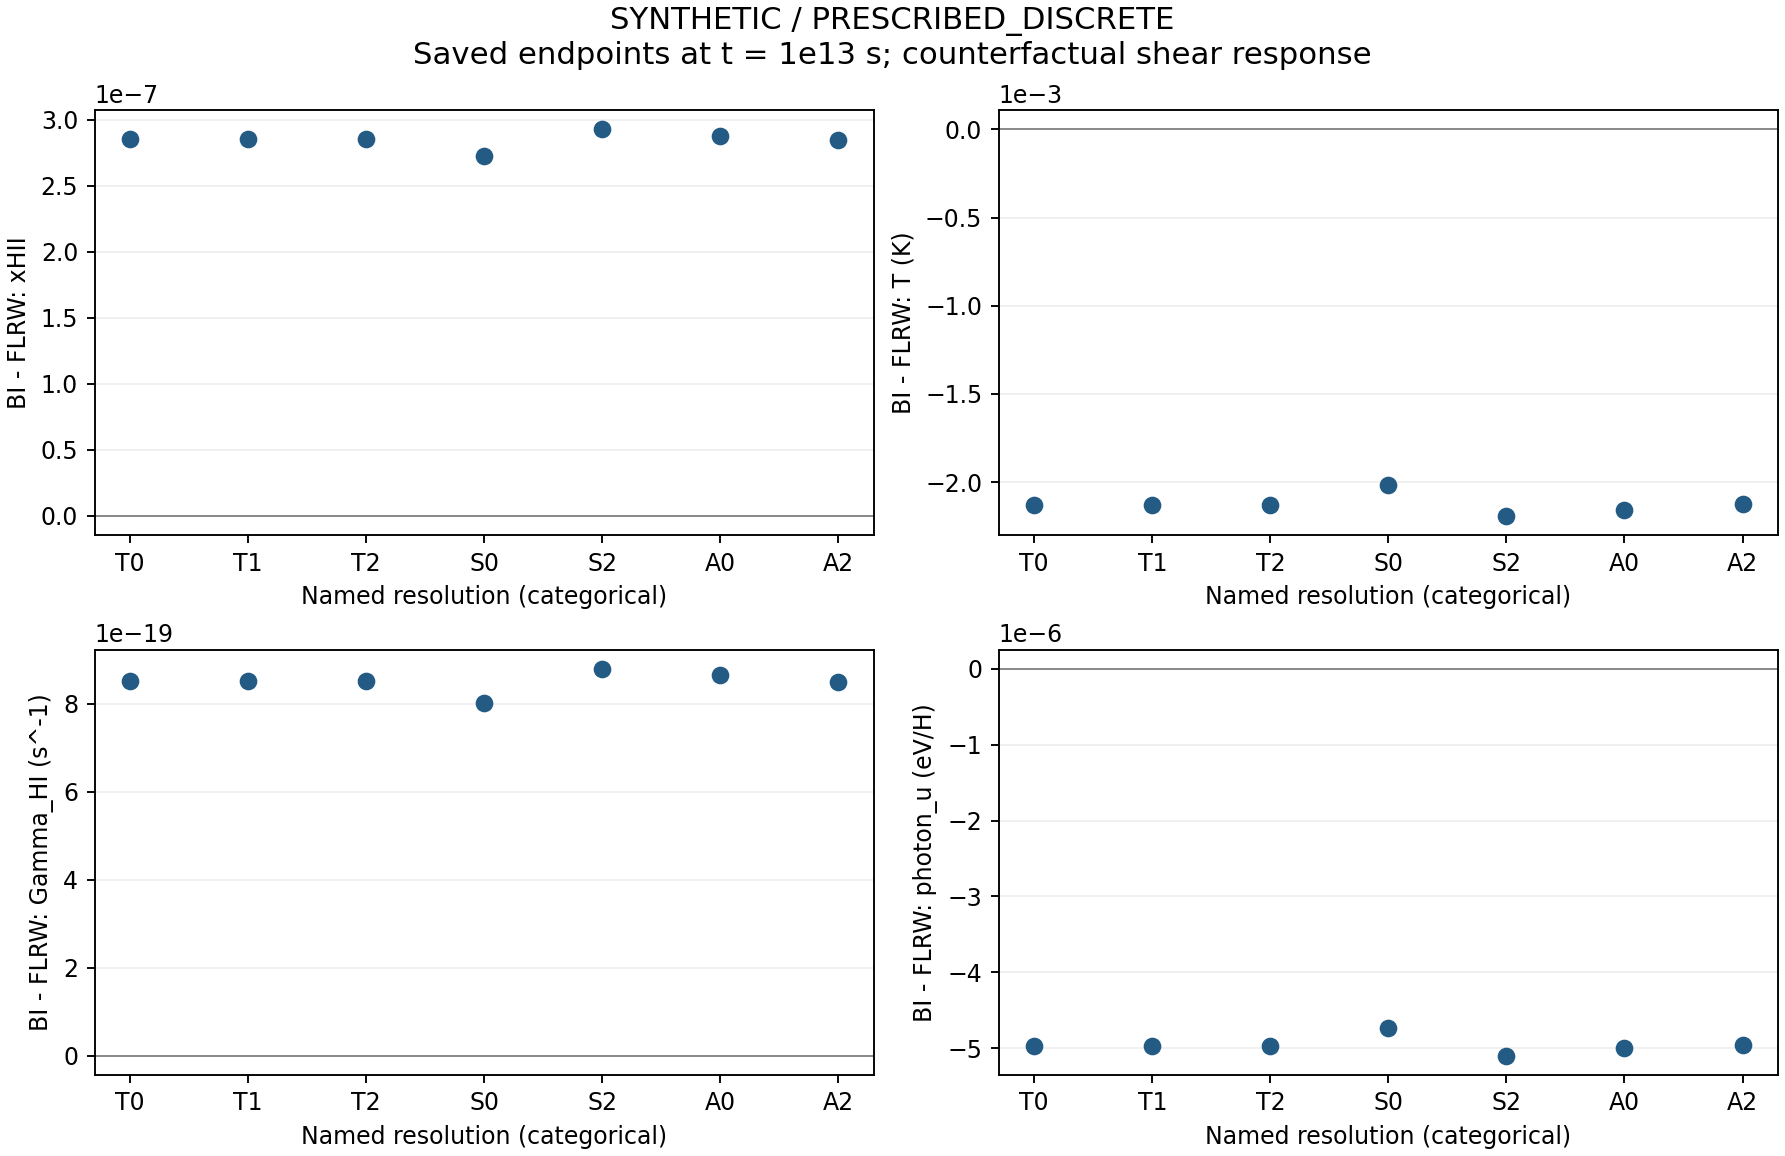
\includegraphics[width=0.96\linewidth]{../../../docs/fastest_track_chat/REI-CODEX-SCIENCE-20261014/retained/endpoint_response.png}
\caption{보존 endpoint의 범주별 BI$-$FLRW 응답. 가로축은 시간축이 아니다.}\end{figure}
\noindent 데이터·그림·receipt의 SHA256 identity와 해석 범위는 함께 제공되는 \texttt{SOURCE\_MANIFEST.json}에 있다. EPS\_HALF/T0 비율은 범위 제한 진단이며 보편적 scaling 정리가 아니다.
\section{claim 경계와 unknown}
\texttt{physical\_fit\_error=NOT\_MEASURED}, \texttt{model\_error=NOT\_MEASURED}, \texttt{continuum\_error\_bound=NOT\_ESTABLISHED}, \texttt{QV=NOT\_EVALUABLE}. 물리적 EoR, full 17-state history, 관측 확률/하늘, 복원 history, 신규 scientific PASS는 주장하지 않는다. unknown tail과 absolute-IVP 값은 null이다. warm provider의 30000--110000 K 범위는 cold EoR domain이 아니며 확대하지 않는다.
\section{대기 중인 결과}
\paragraph{RUX05: 첫 FLRW 구간.} E-P \texttt{coupled\_primary::PrimaryStage} 및 EB warm source는 후보이며 연결과 물리 admission은 미완료다. 배경/clock/origin, gas/radiation IC, emissivity 또는 UVB 역할, 실제 provider domain, closure/event owners와 source assumptions가 결손이다. 실제 RHS 주입 후 positivity, nuclei/charge, photon/energy ledger, residual 및 해당 수렴 검사가 필요하다.
\paragraph{RUX08: FLRW history.} provider/source 유효 범위 내 multi-epoch H/He, 열, photon, segment ledger와 단계별 그림이 대기 중이다. $x_{\rm HII}$는 QV가 아니다.
\paragraph{RUX09: paired history.} RUX07 Bianchi 및 RUX08 FLRW 결과가 없다. 동일 source/clock convention을 쓰고 coupled counterfactual의 $n_e,T$를 각각 풀어야 한다.
\paragraph{RUX10: BASS receiver.} admitted proper $n_e(t)$ interval과 segment $\tau$/visibility가 없다. 물리적 총량은 관측자/clock 및 tail이 있어야 하며 unknown tail을 0으로 둘 수 없다. full paired observable은 RUX09 및 tail 이후에만 가능하다.
\section{갱신 규칙}
새 admitted interval/history/paired/receiver 자료가 생기면 이 문서를 갱신하고 기존 scoped claim 및 실패를 보존한다. 이 draft는 최종 전체 figure/report나 RUX16 과학 admission이 아니다.
\end{document}
